%versi 3 (22-07-2020)
\chapter{Landasan Teori}
\label{chap:teori}

% Reference test
%\cite{mueller:2007:windowscommandline}
%\cite{hill:2009:effectivewindowspowershell}
%\cite{shottsjr:2019:linuxcommandline}
%\cite{matthew:2007:beginninglinuxprogramming}
%\cite{kerrisk:2010:linuxprogramminginterface}

\section{\textit{Command Line}}
\label{sec:commandline}
\textit{Command line} (atau \cli) dapat diartikan sebagai tampilan antarmuka/\textit{interface} yang memproses perintah dari pengguna dan meneruskannya langsung ke sistem operasi untuk dijalankan.\cite{shottsjr:2019:linuxcommandline} Seluruh sistem operasi komputer yang ada memiliki sebuah \cli dalam bentuk \textit{shell}, yang dapat digunakan oleh penggunanya untuk langsung mengakses fungsi atau servis yang disediakan oleh sistem operasi.\cite{mueller:2007:windowscommandline} 

%Sedangkan, perangkat lunak yang memproses \cli ini disebut sebagai \cl \textit{interpreter}\cite{mueller:2007:windowscommandline} atau \textit{shell}.\cite{shottsjr:2019:linuxcommandline}

\subsection{\textit{Command Line Interface} dan \textit{Graphical User Interface}}
\label{sec:commandline-comparison}

Ada beberapa dari tipe antarmuka yang masih banyak digunakan di zaman sekarang, tetapi dua tipe yang paling banyak muncul adalah \cli dan \gui. Perangkat lunak berbasis \cl sendiri bisa memiliki berbagai macam tampilan, tetapi semuanya selalu mengikuti satu bentuk antarmuka umum. Bentuk yang dimaksud adalah sebuah area/\textit{window} yang memuat teks berupa perintah-perintah dari user untuk dilakukan oleh komputer, beserta keluarannya yang juga berupa teks, seperti dapat dilihat pada gambar \ref{fig:commandline-cli}. Jenis perangkat lunak seperti ini disebut memiliki antarmuka jenis \cli (CLI). Adapun dekorasi visual yang dimiliki oleh jenis tampilan ini hanya berupa warna pada teks-teks yang ada, tanpa tambahan gambar apapun. Jika perangkat lunak tersebut memiliki dekorasi dan/atau tombol interaktif berupa gambar grafis, seperti pada gambar \ref{fig:commandline-gui}, maka perangkat lunak tersebut dikategorikan sebagai perangkat lunak berbasis \gui.

\begin{figure}[ht]
    \begin{subfigure}[b]{0.475\linewidth}
		\centering
		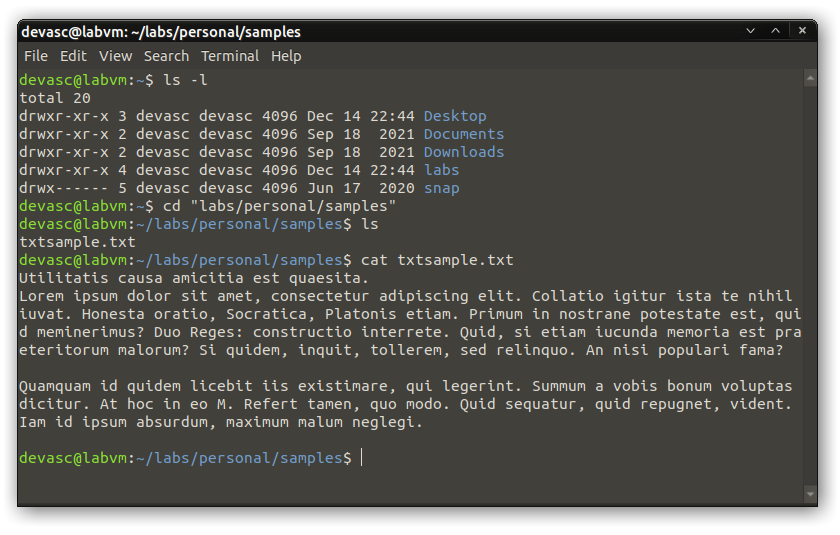
\includegraphics[height=4.7cm]{terminal-linux}
		\caption{Antarmuka perangkat lunak berbasis \cli.}
		\label{fig:commandline-cli}
	\end{subfigure}
	\hfill
    \begin{subfigure}[b]{0.475\linewidth}
		\centering
		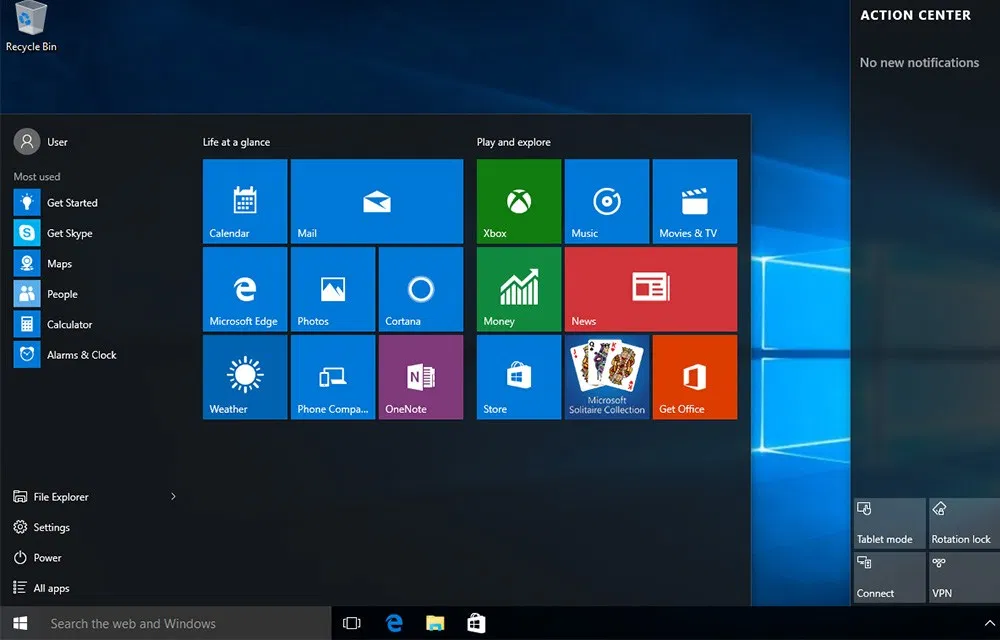
\includegraphics[height=4.5cm]{gui}
		\caption{Antarmuka perangkat lunak berbasis \gui.}
		\label{fig:commandline-gui}
	\end{subfigure}
    \caption[Dua jenis tampilan perangkat lunak]{Contoh dua jenis antarmuka (\textit{interface)} perangkat lunak.}
	\label{fig:commandline-interfacetypes}
\end{figure}

Selain dari tampilannya sendiri, ada beberapa perbedaan utama lain antara perangkat-perangkat lunak berbasis \cli dengan perangkat lunak berbasis \gui. Adapun perbedaan-perbedaan utama dari kedua jenis antarmuka ini adalah sebagai berikut.\cite{mueller:2007:windowscommandline}
\begin{itemize}
	\item Pengunaan sumber daya sistem untuk menjalankan perangkat lunak berbasis \cli lebih rendah dibandingkan dengan perangkat lunak berbasis \gui.
	\item Bagi pengguna pemula (atau pengguna awam pada umumnya), perangkat lunak berbasis \cli akan lebih sulit digunakan karena tidak adanya bantuan apapun dalam bentuk visual, sehingga satu-satunya cara untuk tahu bagaimana cara menggunakan fitur-fiturnya adalah melalui dokumentasi perangkat lunak yang ada. Karena alasan yang sama pula, perangkat lunak berbasis \cli lebih sulit untuk dibiasakan penggunaannya.
	\item Automasi perintah yang bersifat berulan-ulang jauh lebih mudah dilakukan pada perangkat lunak berbasis \cli. Hal ini dikarenakan perangkat lunak berbasis \cli tidak hanya lebih mudah untuk dibuat \textit{script}-nya, tetapi juga lebih efisien untuk digunakan ketika ada banyak sekali perintah yang harus dilakukan pada suatu saat tertentu.
\end{itemize}

\subsection{\textit{Command Line} di Linux}
\label{sec:commandline-linux}

Linux merupakan sebuah sistem operasi yang sangat modular, jadi ada banyak sekali \textit{shell} yang dapat dijalankan dan digunakan di dalamnya. Walaupun begitu, ada satu \textit{shell} yang selalu datang ter-\textit{install} di dalam semua sistem operasi Linux, yaitu \textit{``bash"} (GNU \textit{\textbf{B}ourne \textbf{A}gain \textbf{Sh}ell}).\cite{matthew:2007:beginninglinuxprogramming}

\subsubsection{Tampilan}
\label{sec:commandline-linux-appearance}

Ketika terminal di Linux dijalankan, akan keluar kotak dialog, beserta sebuah baris. Baris ini biasanya berisi sebuah teks dengan format sebagai berikut.

\begin{verbatim}
        <nama pengguna>@<nama perangkat>:<direktori yang sedang diproses>$
\end{verbatim}

Tanda dolar di ujung baris ini menandakan bahwa baris tersebut merupakan baris \textit{shell prompt}, yang merupakan waktu di mana terminal sudah siap menerima masukan dari pengguna untuk diproses. Perlu diingat bahwa di posisi tanda dolar ini, terkadang justru terdapat tanda pagar (\#). Tanda pagar di akhir baris \textit{shell prompt} menandakan bahwa terminal tersebut dijalankan dengan tingkat akses \textit{superuser}, yang berarti bahwa entah pengguna masuk ke sistem sebagai user \textit{root}, atau terminal memiliki izin tingkat \textit{superuser/administrator}.\cite{shottsjr:2019:linuxcommandline}

\begin{figure}[ht]
    \begin{subfigure}[b]{0.475\linewidth}
		\centering
		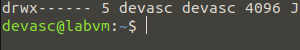
\includegraphics[width=\linewidth]{linux-shellprompt-normal}
		\caption{\textit{Shell prompt} terminal dengan tingkat izin \mbox{normal}.}
		\label{fig:shellprompt-linux-normal}
	\end{subfigure}
	\hfill
    \begin{subfigure}[b]{0.475\linewidth}
		\centering
		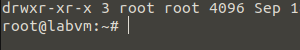
\includegraphics[width=\linewidth]{linux-shellprompt-superuser}
		\caption{\textit{Shell prompt} terminal dengan tingkat izin \textit{\mbox{superuser}}.}
		\label{fig:shellprompt-linux-superuser}
	\end{subfigure}
    \caption{Baris \textit{shell prompt} terminal di sistem operasi Linux.}
	\label{fig:commandline-shellprompt-linux}
\end{figure}

\subsubsection{Navigasi \cite{shottsjr:2019:linuxcommandline}}
\label{sec:commandline-linux-nav}

Sama seperti di Windows, Linux menyimpan file-filenya di sebuah struktur direktori yang bersifat hierarkial. Hal ini berarti bahwa file-file tersebut disimpan dalam direktori-direktori (atau \textit{folder-folder}) yang tersusun seperti sebuah pohon. dalam arti bahwa satu \textit{folder} bisa jadi berada di dalam satu \textit{folder} lain, atau berisi beberapa \textit{folder} lainnya.

Untuk navigasi, terminal Linux memiliki beberapa perintah utama. Adapun perintah-perintah tersebut adalah sebagai berikut.

\begin{itemize}
	\item \verb|pwd|\\
	\verb|pwd| merupakan singkatan dari \textit{print working directory}, yang berarti bahwa perintah ini akan mengeluarkan \textit{working directory}, atau direktori tempat terminal sekarang sedang bekerja/berjalan, sebagai keluaran dari perintah tersebut. Ketika pengguna pertama kali menjalankan terminal, \textit{working directory}-nya selalu merupakan direktori \textit{home} dari perangkat.
	\item \verb|ls|\\
	\verb|ls| digunakan untuk menghasilkan keluaran berupa isi dari folder yang dispesifikasi. Biasanya digunakan ketika pengguna sudah memasuki folder yang diinginkan, walaupun dengan perintah ini, pengguna bisa saja mengintip isi dari folder manapun di direktori manapun, dengan mengikutkan direktori yang diinginkan sebagai parameter dari perintah tersebut. Adapun Isi dari folder yang diikutkan sebagai parameter tidak hanya berupa folder lain, tetapi juga seluruh file-file yang ada, walaupun untuk file-file yang disembunyikan (nama file diawali dengan tanda titik), perlu ditambahkan opsi \verb|-a| agar file-file tersebut muncul pula dalam keluarannya.
	\item \verb|cd|\\
	\verb|cd| adalah perintah yang berfungsi untuk mengganti \textit{working directory} dari terminal. Untuk melakukan hal tersebut, perintah yang perlu dimasukkan adalah sebagai berikut:
	
	\begin{verbatim}
	                     cd <direktori yang diinginkan>
	\end{verbatim}
	
	Direktori yang diinginkan dapat berupa direktori absolut, atau direktori relatif. Perbedaannya adalah direktori absolut selalu dimulai dari folder \textit{root}, mengikuti folder-folder apapun yang ada di antara \textit{root} sampai ke folder yang diinginkan.
	
	Sedangkan, direktori relatif selalu dimulai dari \textit{working directory}. Untuk penggunaan direktori relatif, diperlukan dua buah notasi spesial, yaitu titik (\verb|.|), yang merepresentasikan \textit{working directory} sekarang itu sendiri, dan dua titik (\verb|..|), yang merepresentasikan \textit{parent folder} dari \textit{working directory}.
\end{itemize}

\subsection{\textit{Command Line} di Windows}
\label{sec:commandline-windows}

Cara kerja \cl di Windows serupa dengan cara kerja \cl di Linux, dalam arti bahwa untuk bekerja dengan \cl di Windows, penggunanya juga akan langsung berinteraksi dengan utilitas yang disediakan oleh sistem operasi. \textit{Command line} di Windows juga dapat digunakan untuk hal-hal yang serupa dengan \cl di Linux, seperti menulis (dan menjalankan) \textit{script}, menjalankan perintah yang diinginkan pengguna secara otomatis, atau melihat status dari sistem operasi.\cite{mueller:2007:windowscommandline}

Masih sama dengan Linux, ada banyak sekali command yang bisa digunakan, sehingga susah untuk menghafal seluruh command-command yang ada\textemdash termasuk masukan, parameter-parameter yang dibutuhkan, serta keluarannya. Untuk melihat dokumentasi, atau penjelasan detail untuk masukan, keluaran, parameter, serta opsi-opsi dari perintah tertentu, pengguna dapat memasukkan perintah tersebut, diikuti dengan \verb|/?|.\cite{mueller:2007:windowscommandline}

\subsubsection{Tampilan}
\label{sec:commandline-windows-appearance}

Di sistem operasi Windows, ada dua jenis antarmuka \cl, yaitu cmd (\textit{Command Prompt}) dan \textit{PowerShell}. Keduanya memiliki tampilan yang kurang lebih sama\textemdash hanya saja awalnya cmd memiliki latar belakang hitam, sedangkan \textit{PowerShell} memiliki latar belakang biru tua, seperti terlihat di gambar \ref{fig:commandline-windows-programs}.

\begin{figure}[ht]
    \begin{subfigure}[b]{0.49\linewidth}
		\centering
		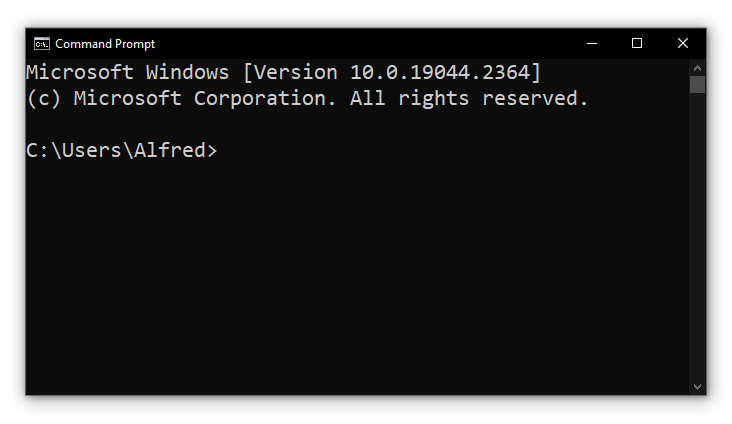
\includegraphics[width=\linewidth]{windows-cmd}
		\caption{Antarmuka Windows \textit{Command Prompt} (\textit{cmd})}
		\label{fig:commandline-windows-cmd}
	\end{subfigure}
	\hfill
    \begin{subfigure}[b]{0.49\linewidth}
		\centering
		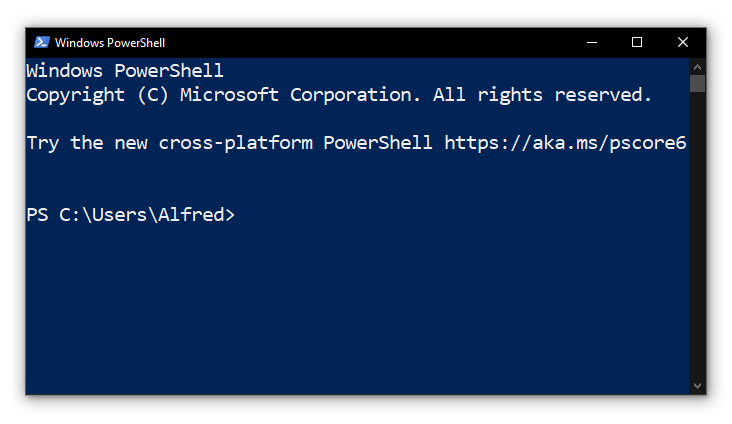
\includegraphics[width=\linewidth]{windows-powershell}
		\caption{Antarmuka Winodws \textit{PowerShell}}
		\label{fig:commandline-windows-powershell}
	\end{subfigure}
    \caption{Tampang kedua antarmuka \cl bawaan di sistem operasi Windows.}
	\label{fig:commandline-windows-programs}
\end{figure}

\subsubsection{Navigasi}
\label{sec:commandline-windows-nav}

Untuk navigasi di antarmuka \cl Windows, ada dua perintah penting yang dipakai ketika pengguna sedang berurusan dengan file-file dan navigasi dalam direktori sistem. Kedua perintah tersebut adalah \verb|cd| dan \verb|dir|.

\begin{itemize}
	\item \verb|cd| (\verb|chdir|)\footnote{\href{https://docs.microsoft.com/en-us/windows-server/administration/windows-commands/cd}{cd | Microsoft Docs}}\\
	\verb|cd| merupakan sebuah perintah yang memiliki tiga fungsi utama, yaitu menampilkan \textit{drive} tempat sedang \cl berada (jika pengguna hanya memasukkan \verb|cd| tanpa parameter apapun), menampilkan direktori tempat \cl sedang berada (jika pengguna hanya memasukkan \textit{drive} sebagai parameter, atau fungsi yang paling umumnya, untuk mengganti \textit{working directory} dari \cl.
	\newline\newline
	Adapun format dari perintah \verb|dir| adalah sebagai berikut.
	
	\begin{verbatim}
                        cd [/d] [<drive>:][<path>]
	\end{verbatim}
	
	\newpage % Preventing widow
	Dengan fungsi dari semua opsi dan parameter yang ada sebagai berikut.
	
	\begin{itemize}
		\item \verb|/d|\\
		Opsi yang menandakan bahwa pengguna ingin mengganti \textit{drive} (partisi) dan juga \textit{working directory} dari \cl.
		\item \verb|<drive>:|\\
		Kode huruf dari partisi yang akan diproses.
		\item \verb|<path>|\\
		Direktori yang akan diproses. Parameter ini harus diikutkan beserta kode huruf partisi (tidak dapat berdiri sendiri.)
	\end{itemize}
	
	\item \verb|dir|\\
	\verb|dir| merupakan sebuah perintah yang mengeluarkan/menampilkan sebuah daftar berisi file-file yang ada di suatu direktori, termasuk subdirektori. Jika tidak disertai parameter apapun, perintah ini akan menampilkan label volume dan nomor serial \textit{disk}, dilanjutkan dengan daftar direktori dan file di dalamnya. Untuk file, akan ditampilkan nama beserta ukurannya. Perintah ini juga akan menampilkan jumlah direktori dan file yang didaftarkan, ukuran kumulatifnya, dan sisa dari \textit{disk} yang tidak terpakai (dalam \textit{bytes}).\footnote{\href{https://docs.microsoft.com/en-us/windows-server/administration/windows-commands/dir}{dir | Microsoft Docs}}
	\newline\newline
	Adapun format dari perintah \verb|dir| adalah sebagai berikut.\cite{mueller:2007:windowscommandline}
	
	\begin{verbatim}
dir [drive:][path][filename] [/A[[:]attributes]] [/B] [/C] [/D] [/L] [/N] 
[/O[[:]sortorder]] [/P] [/Q] [/R] [/S] [/T[[:]timefield]] [/W] [/X] [/4]
	\end{verbatim}
	
	Untuk perintah ini, seperti terlihat di atas, memiliki banyak sekali opsi dan parameter. Tiap-tiap dari parameter tersebut memiliki fungsi tersendiri, yaitu:
	\begin{itemize}
		\item \verb|/A[[:]attributes]|\\
		Menampilkan file-file dengan atribut tertentu, seperti file yang disembunyikan, file sistem, file \textit{read-only}, dan sebagainya.
		\item \verb|/B|\\
		Menghilangkan \textit{heading} dan ringkasan informasi dari keluaran, atau dengan kata lain, hanya menampilkan file-file dan direktori, tanpa informasi tambahan apapun.
		\item \verb|/C|\\
		Menggunakan separator koma untuk tiap angka ribuan di ukuran file. Jika opsi yang dimasukkan adalah \verb|/-C|, separator koma justru akan dihilangkan.
		\item \verb|/D|\\
		Menampilkan keluaran dengan format yang lebih lebar. Jika opsi ini diikutkan, keluaran akan ditampilkan dengan urutan berdasarkan kolom.
		\item \verb|/L|\\
		Seluruh teks dalam keluaran akan menggunakan huruf kecil. Jika opsi ini tidak digunakan, keluaran akan mengandung huruf besar dan huruf kecil \textit{mixed case}.
		\item \verb|/N|\\
		Menampilkan daftar dengan format panjang, dengan nama file berada di ujung paling kanan.
		\newpage \enlargethispage{1.5\baselineskip} % Preventing widow
		\item \verb|/O[[:]sortorder]|\\
		Menampilkan daftar direktori yang terurut berdasarkan urutan tertentu, seperti berdasarkan ekstensi file, berdasarkan tanggal dibuat, berdasarkan nama, dan sebagainya. Jika tidak diikutkan tanda minus (\verb|-|) sebelum huruf \verb|O| pada perintah, daftar yang muncul akan terurut secara menaik.
		\item \verb|/P|\\
		Memberhentikan keluaran selama beberapa waktu singkat (memberi jeda kecil) setelah setiap halaman informasi.
		\item \verb|/Q|\\
		Menambahkan informasi mengenai pemilik file dalam keluaran.
		\item \verb|/R|\\
		Menampilkan \textit{data stream} alternatif, jika ada.
		\item \verb|/S|\\
		Mendaftarkan seluruh file di direktori dan subdirektori yang diproses. Tiap-tiap direktori akan memiliki \textit{header} tersendiri dalam keluarannya.
		\item \verb|/T[[:]timefield]|\\
		Menspesifikasi \textit{time field} mana yang akan tampil dan digunakan sebagai urutan, jika aturan pengurutan lain tidak ditentukan. \textit{Time field} yang dapat digunakan adalah waktu pembuatan file, kapan terakhir file diakses, dan kapan file terakhir dimodifikasi. Jika parameter ini tidak dispesifikasi, \textit{time field} yang digunakan adalah kapan file terakhir dimodifikasi.
		\item \verb|/W|\\
		Menampilkan keluaran dengan format yang lebih lebar. Opsi ini hampir sama dengan \verb|/D|, hanya saja untuk \verb|/W|, jika opsi ini diikutkan, keluaran akan ditampilkan dengan urutan berdasarkan baris, dan bukan kolom.
		\item \verb|/X|\\
		Menampilkan nama pendek yang dibuat untuk nama-nama file non-8.3. Opsi ini memiliki format taampilan yang sama seperti opsi \verb|/N|, hanya saja nama pendeknya ditampilkan di keluaran sebelum nama panjangnya.
		\item \verb|4|\\
		Menampilkan angka tahun dengan format angka empat digit.
	\end{itemize}
\end{itemize}

\section{KIRI}
\label{sec:kiri}

KIRI merupakan sebuah perangkat lunak berbasis web yang berfungsi untuk menyelesaikan (atau setidaknya mengurangi) dampak dari masalah-masalah yang dapat diselesaikan oleh transportasi umum/publik di Indonesia, seperti pemanasan global, kemacetan, atau peningkatan harga bensin. Selain itu, turis mancanegara juga memilih untuk menaiki transportasi umum, karena jenis sarana transportasi tersebut tidak hanya jauh lebih murah, tetapi juga memberikan kesempatan yang mudah kepada mereka untuk melihat seluk-beluk dari kota-kota yang mereka kunjungi. Walaupun begitu, banyak masyarakat lokal sendiri yang seringkali masih segan untuk menaiki transportasi publik, umumnya karena transportasi publik dianggap lebih rumit persiapannya dibandingkan dengan metode-metode transportasi privat, seperti menaiki kendaraan pribadi.\footnote{\href{https://projectkiri.github.io/\#about-kiri}{https://projectkiri.github.io/\#about-kiri}}

Di halaman web KIRI, pengguna dapat memasukkan input berupa lokasi awal dan lokasi tujuan dan KIRI akan menghasilkan seluruh langkah yang harus ditempuh oleh pengguna untuk sampai ke lokasi tujuan, dengan menggunakan angkot. Keluaran ini sudah meliputi kode angkot mana saja yang harus dinaiki, dan juga seberapa jauh pengguna harus berjalan kaki untuk sampai ke lokasi rute angkot berikutnya.

\subsection{Tampilan}
\label{sec:kiri-appearance}

Pada saat pertama kali dibuka, hal pertama yang paling mencolok di halaman awal web KIRI adalah sebuah peta besar di sebelah kiri yang dapat diperbesar ataupun diperkecil. Sedangkan, bagian kanan dari halamannya terdiri atas beberapa bagian. Di bagian paling atas terdapat logo KIRI, beserta sepasang menu \textit{dropdown}\textemdash yang pertama merupakan pilihan kota tempat pengguna berada (untuk sekarang hanya tersedia pilihan kota Jakarta dan Bandung), dan yang kedua merupakan pilihan bahasa, entah bahasa Indonesia atau Inggris. Di bawahnya merupakan sepasang menu \textit{dropdown} yang merupakan tempat di mana pengguna memasukkan lokasi awal dan tujuan yang akan diproses oleh KIRI. Terakhir, di bawahnya ada sebuah bagian kosong, yang nantinya akan menjadi tempat di mana KIRI akan meletakkan keluaran dari prosesnya. Adapun tampilan awal dari halaman web ini dapat dilihat di gambar \ref{fig:kiri-base}.

\begin{figure}[ht]
    \centering
    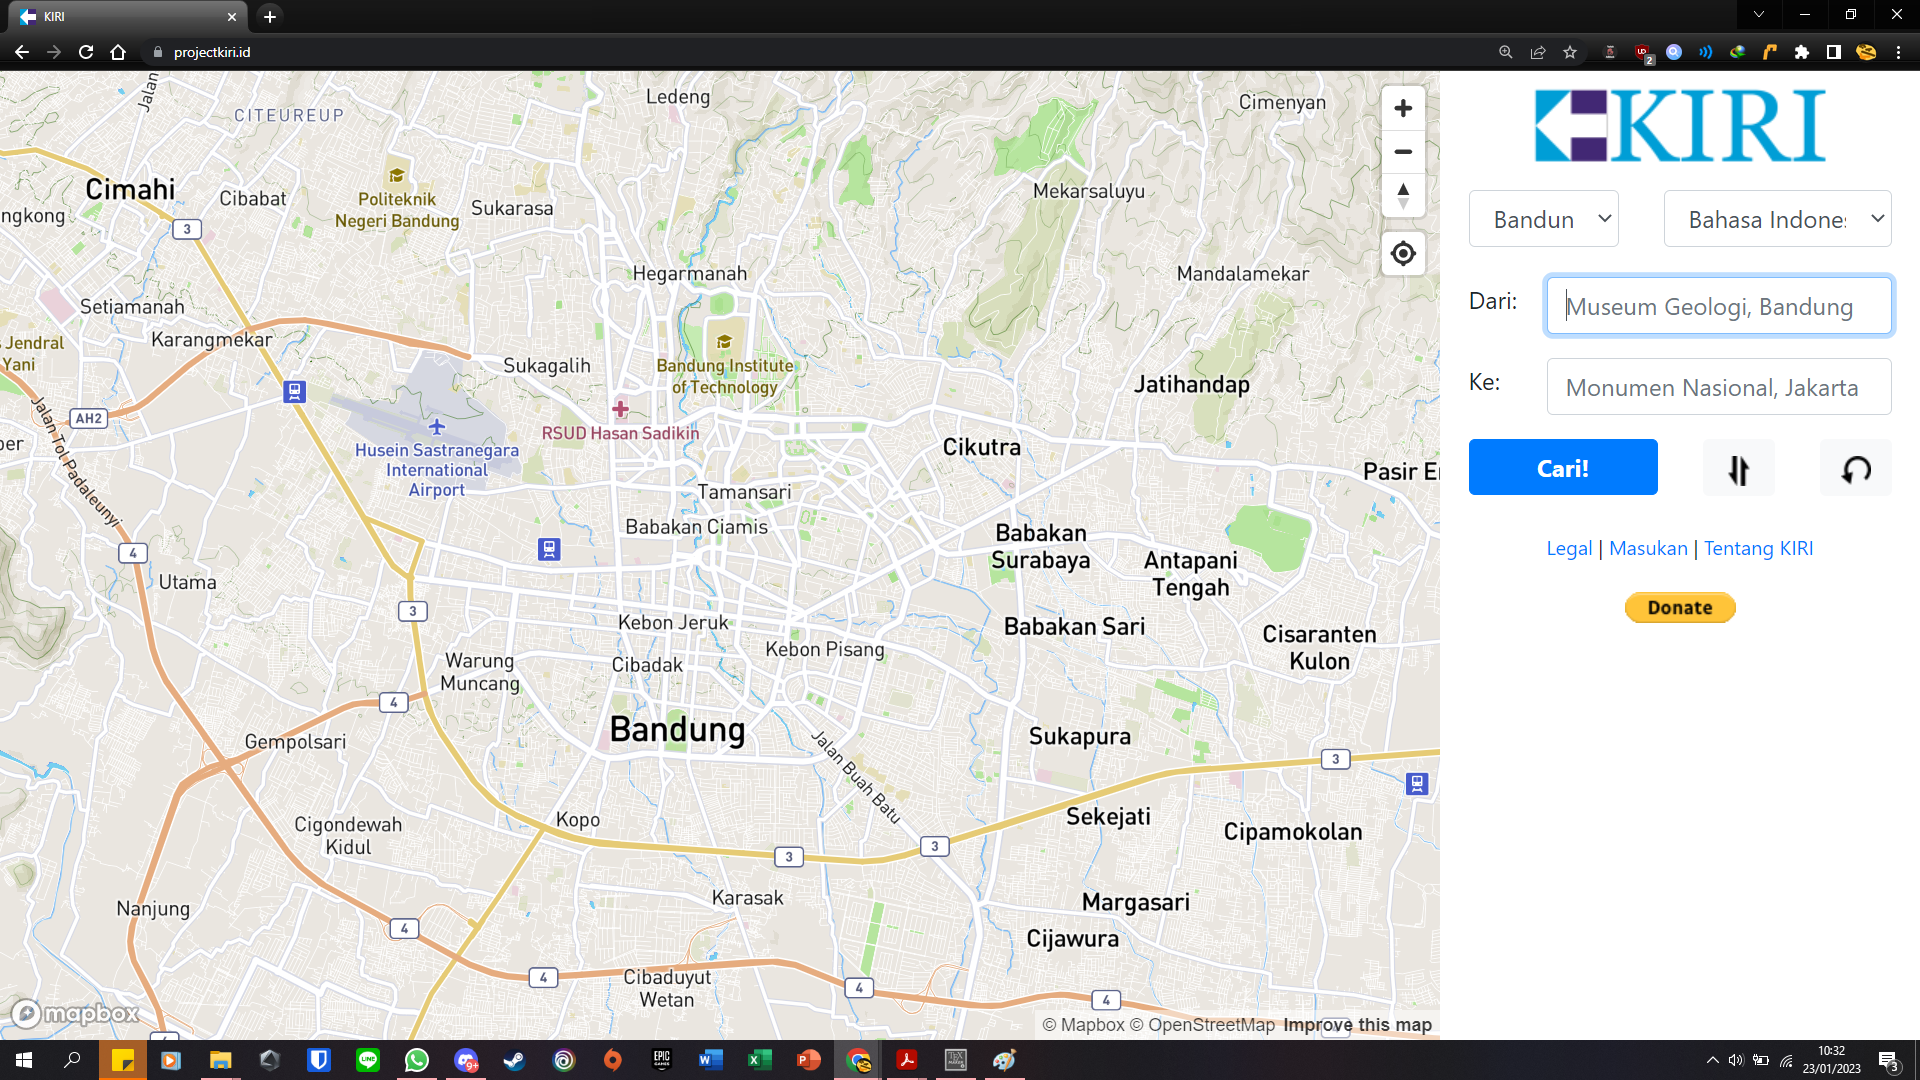
\includegraphics[width=0.74\linewidth]{projectkiri-base}
    \caption[Tampilan awal halaman web KIRI]{Tampilan awal halaman web KIRI.}
    \label{fig:kiri-base}
\end{figure}

Ada dua area yang memiliki perbedaan yang signifikan ketika pengguna sudah memasukkan masukan dan menyuruh KIRI untuk memprosesnya. Bagian yang pertama adalah bagian peta, yang setelah pemrosesan masukan, akan memiliki garis-garis berwarna yang menandakan rute angkot maupun tujuan perjalanan kaki yang harus ditempuh oleh pengguna. Bagian kedua adalah bagian keluaran, yang tadinya kosong, sekarang akan berisi langkah-langkah yang harus ditempuh oleh penggunanya untuk pergi dari lokasi awal ke lokasi tujuan. Spesifiknya, perbedaan-perbedaan ini dapat dilihat di gambar \ref{fig:kiri-example}.

\begin{figure}[ht]
    \centering
    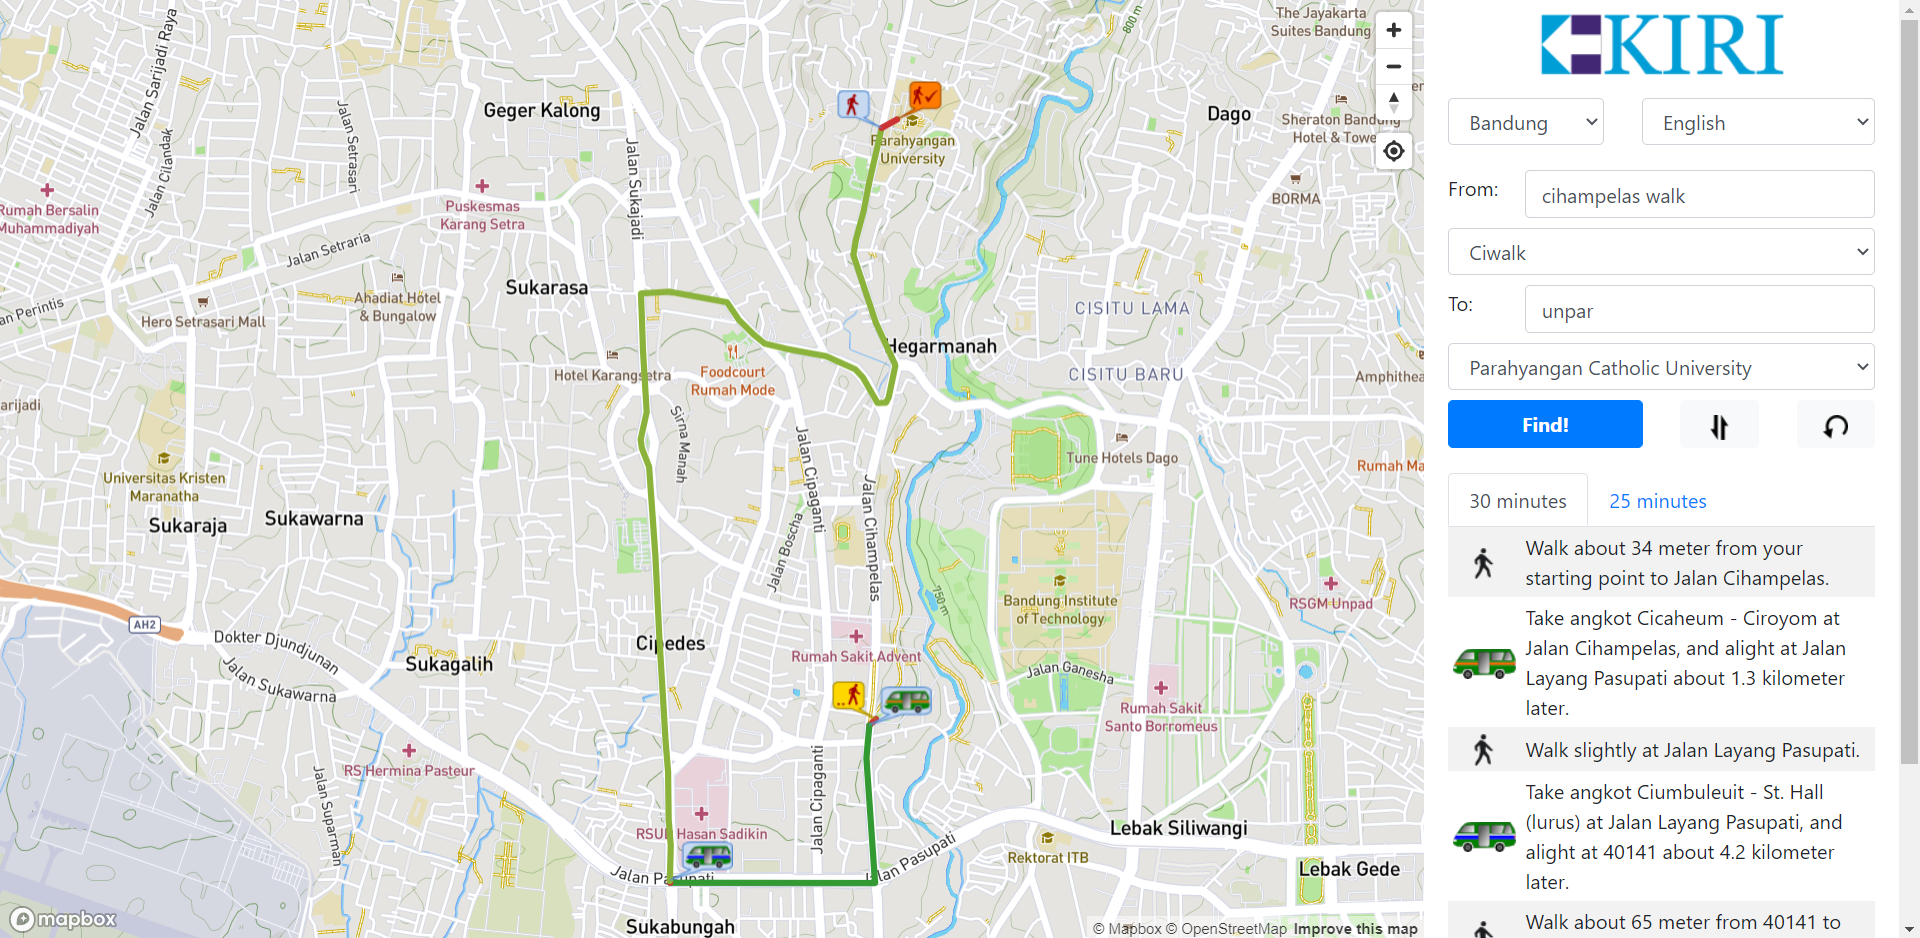
\includegraphics[width=0.74\linewidth]{projectkiri-example}
    \caption[Tampilan akhir halaman web KIRI]{Tampilan halaman web KIRI setelah pemrosesan masukan dari pengguna selesai.}
    \label{fig:kiri-example}
\end{figure}

\subsection{API}
\label{sec:kiri-api}

KIRI juga memiliki sebuah API yang dapat digunakan untuk keperluan pengembangan perangkat lunak. Seluruh permintaan (\textit{request}) yang dilakukan melalui API KIRI harus dilakukan sebagai permintaan tipe GET ke \href{https://projectkiri.id/api}{https://projectkiri.id/api}, beserta parameter-parameter yang dibutuhkan. 
\newline\newline
Permintaan tersebut harus memiliki parameter-parameter seperti terlihat di bawah ini.\footnote{\href{https://github.com/projectkiri/Tirtayasa/wiki/KIRI-API-v2}{https://github.com/projectkiri/Tirtayasa/wiki/KIRI-API-v2}}

\begin{itemize}
	\item \verb|version|\\
	\textbf{Kemungkinan nilai:} \verb|2|\\
	Parameter ini merupakan tanda bagi API untuk menggunakan protokol versi 2.
	\item \verb|mode|\\
	\textbf{Kemungkinan nilai:} \verb|findroute|\\
	Parameter ini merupakan mode dari servis/jasa API yang akan digunakan oleh pengguna. Untuk mode \verb|findroute|, jasa yang akan digunakan adalah jasa pencarian rute dengan angkot.
	\item \verb|locale|\\
	\textbf{Kemungkinan nilai:} \verb|en| atau \verb|id|\\
	Parameter ini mengatur bahasa apa yang akan digunakan dalam keluaran API nantinya\textemdash\verb|en| berarti keluaran akan menggunakan bahasa Inggris, dan \verb|id| berarti keluaran akan menggunakan bahasa Indonesia.
	\item \verb|start|\\
	\textbf{Kemungkinan nilai:} \verb|lat|, \verb|lng|; dalam bentuk desimal\\
	Parameter ini merupakan nilai \latlon dari titik awal perjalanan pengguna.
	\item \verb|finish|\\
	\textbf{Kemungkinan nilai:} \verb|lat|, \verb|lng|; dalam bentuk desimal\\
	Parameter ini merupakan nilai \latlon dari titik akhir/tujuan perjalanan pengguna.
	\newpage % Preventing widow
	\item \verb|presentation|\\
	\textbf{Kemungkinan nilai:} \verb|desktop|\\
	Parameter ini hanya digunakan untuk fitur \textit{backwards compatibility}.
	\item \verb|apikey|\\
	\textbf{Kemungkinan nilai:} angka heksadesimal 16-digit\\
	Parameter ini berisi kunci API pribadi yang harus digenerasi terlebih dahulu sebelum API dapat digunakan.
\end{itemize}
\vspace{\baselineskip}
Sedangkan, respon yang diberikan oleh API berupa sebuah objek JSON yang selalu memiliki setidaknya dua variabel, yaitu:\footnote{\href{https://github.com/projectkiri/Tirtayasa/wiki/KIRI-API-v2}{https://github.com/projectkiri/Tirtayasa/wiki/KIRI-API-v2}}

\begin{itemize}
	\item \verb|status|\\
	\textbf{Kemungkinan nilai:} \verb|ok| atau \verb|error|\\
	Variabel ini manandakan apakah permintaan berhasil diproses atau tidak. Jika permintaan berhasil diproses, variabel ini akan bernilai \verb|ok|, dan jika tidak, variabel ini akan bernilai \verb|error|.
	\item \verb|message|\\
	Variabel ini bisa berisi dua macam objek. Jika permintaan dari user tidak berhasil diproses, atau dalam kata lain, terjadi sebuah \textit{error}, maka variabel ini akan berisi string yang merupakan pesan \textit{error} serta alasan spesifik mengapa \textit{error} tersebut terjadi. Di lain sisi, jika permintaan dari user berhasil diproses, variabel ini akan mengalami dua perubahan utama. Pertama, nama variabel ini akan berubah menjadi \verb|routingresults|, dan kedua, isi dari variabel ini akan menjadi sebuah \textit{array} JSON yang merupakan respon dari API KIRI berupa keluaran yang akan dilihat oleh pengguna. \textit{Array} JSON ini sendiri terbagi menjadi beberapa variabel lainnya, yang dapat dilihat di daftar di bawah ini.
	
	\begin{itemize}
		\item \verb|steps|\\
		\textbf{Tipe:} array\\
		Variabel ini merepresentasikan satu buah langkah yang harus ditempuh oleh pengguna. Adapun \textit{array} ini sendiri berisi variabel-variabel berikut:
		
		\begin{itemize}
			\item Tipe transportasi\\
			Tipe sarana transportasi yang harus dipakai oleh pengguna. Jika pengguna harus berjalan kaki, variabel ini akan berisi \verb|walk|. Jika pengguna harus menaiki angkot, variabel ini akan berisi \verb|angkot|.
			\item Kode angkot\\
			Variabel ini menunjukkan angkot mana yang harus dinaiki oleh pengguna di langkah tersebut. Jika penggunaan angkot tidak dimungkinkan pada langkah ini (pengguna harus berjalan kaki), variabel ini akan berisi \verb|walk|.
			\item Array \latlon lokasi\\
			\textit{Array} nilai-nilai desimal \latlon dari berbagai titik lokasi yang terdapat dalam rute.
			\item Deskripsi langkah\\
			Deskripsi langkah yang harus ditempuh, dalam bahasa natural. Bahasa yang digunakan tergantung parameter \verb|locale| yang diatur dalam masukan.
			\item URL untuk mendapatkan tiket kendaraan\\
			Tautan untuk mendapatkan tiket angkutan umum, jika diperlukan. Jika transportasi pada langkah tersebut tidak memerlukan tiket, variabel ini akan berisi \verb|null|.
			\item URL editor rute\\
			Tautan untuk meng-edit rute, jika situasinya memungkinkan. Jika tidak, variabel ini akan berisi \verb|null|.
		\end{itemize}
		
		\item \verb|traveltime|\\
		\textbf{Tipe:} string\\
		Variabel ini berisi estimasi jangka waktu yang diperlukan untuk menyelesaikan langkah tersebut.
	\end{itemize}
	
\end{itemize}
